\documentclass[resume]{subfiles}


\begin{document}
\begin{multicols}{3}
\section{Opamp 2}
\subsection{Suppositions}
\begin{tabular}{p{6cm}c}
Chute de tension dans les sources de courant & \SI{1}{\volt}\\
Chute dans les jonctions (transistors et diodes) & \SI{0.6}{\volt}\\
Tension thermique (résistances) & \SI{25}{\milli\volt}\\
Courant dans la base (à vérifier) & \SI{0}{\ampere}
\end{tabular}
\subsection{Plage d'entrée / de sortie}
Partir du point demandé (entrée ou sortie) et recherche le chemin "logique" qui fait perdre le plus de tension (passage par des transistors/diodes/sources de courant). Il est possible d'utiliser des tensions qui sont écrites sur le schéma.
\begin{figure}[H]
\centering
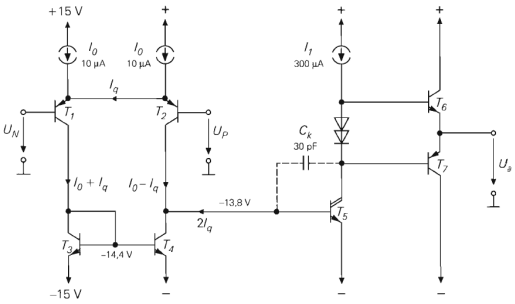
\includegraphics[width=\columnwidth]{img_52.png}
\end{figure}
$$U_N\in\begin{pmatrix}13.4\\ \cancel{-14.4}-13.8\end{pmatrix}\quad U_P\in\begin{pmatrix}13.4\\-13.8\end{pmatrix}\quad U_a\in\begin{pmatrix}13.4\\-13.2\end{pmatrix}$$
Pour les signaux différentiels, ils doivent être identiques donc on utilise la plage la plus faible pour chaque borne.\\
Le \SI{-14.4}{\volt} (à gauche sur le schéma) viens d'une chute de tension de jonction NPN. Le \SI{-13.8}{\volt} (au milieu en bas sur le schéma) viens de la chute de tension double dans le darlington.
$$U_D=U_P-U_N$$
$$I_q=\frac{U_D}{2r_E'}\qquad r_E'=\frac{U_T}{I_0}$$
La tension $U_1$ est entre la base de $T_5$ et la masse.
$$U_1=-2R_1I_q$$
$$U_a=-U_1\frac{R_2}{r_{s5}}$$
$$f_0\approx \frac{1}{2\pi R_1C_k}\cdot \frac{r_{s5}}{R_2}=\SI{5.3}{\hertz}$$
$$S_R=\frac{I_1}{C_k}=\SI{10}{\volt\per\micro\second}$$
$$A=2\frac{R_1R_2}{2r'_E\frac{1}{0.005}}=400'000$$
$$\text{GBW}=A2\pi f_0$$
$$A_{max}=\frac{\text{GBW}}{2\pi \cdot 10'000}=212$$
\subsection{Amplificateur à transconductance}
$$S_D=\frac{I_0}{2U_T}\ \left[\si{\ampere\per\volt}\right]$$
Possibilité de modifier la transconductance en ajoutant une résistance $R_E$ entre les émetteurs de l'étage différentiel.\\
Résistance de sortie :
$$r_a=r_{CE\ 4}$$
\begin{center}
\begin{figure}[H]
\centering
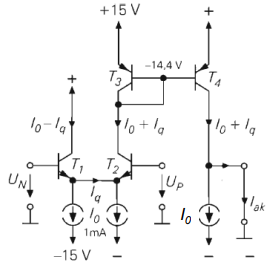
\includegraphics[width=5.00cm]{img_53.png}
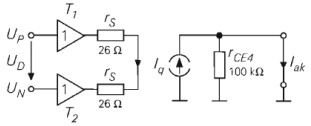
\includegraphics[width=5.00cm]{img_54.png}
\end{figure}
\end{center}
\subsection{Amplificateur à transimpédance}
\begin{figure}[H]
\centering
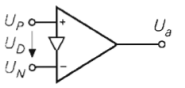
\includegraphics[width=3.00cm]{img_57.png}
\end{figure}
\begin{figure}[H]
\centering
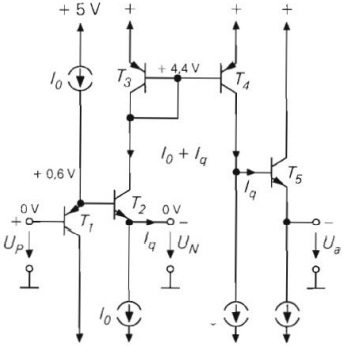
\includegraphics[width=5cm]{img_56.png}
\end{figure}
$$A_D=\frac{U_a}{U_D}=\frac{Z}{r_s}=\frac{U_A}{U_T}$$
\begin{figure}[H]
\centering
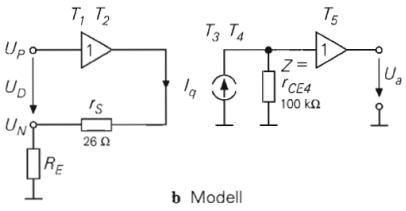
\includegraphics[width=6.00cm]{img_58.png}
\end{figure}
$$A_B=\frac{Z}{R_E+r_s}$$
\subsection{Amplificateur de courant (transistor diamant)}
\begin{figure}[H]
\centering
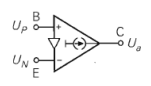
\includegraphics[width=3.00cm]{img_60.png}
\end{figure}
\begin{figure}[H]
\centering
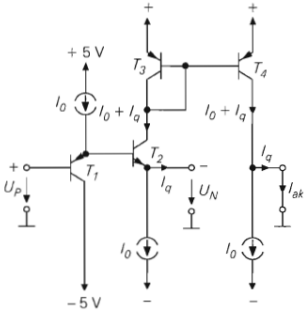
\includegraphics[width=5.00cm]{img_59.png}
\end{figure}
$$S=\frac{1}{r_S}$$
Si on a une résistance externe $R_E$ à l'émetteur 
$$S_B=\frac{1}{r_S+R_E}$$
$$A_B=S_BR=\frac{R}{r_S+R_E}$$
\begin{figure}[H]
\centering
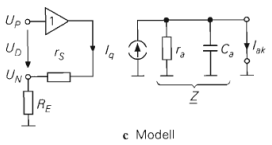
\includegraphics[width=5.00cm]{img_61.png}
\end{figure}
\subsubsection{Couplage sur l'émetteur}
\begin{figure}[H]
\centering
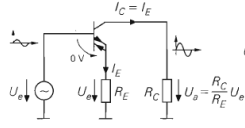
\includegraphics[width=5.00cm]{img_62.png}
\end{figure}
\begin{figure}[H]
\centering
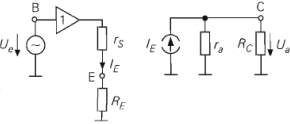
\includegraphics[width=5.00cm]{img_63.png}
\end{figure}
\subsubsection{Couplage sur le collecteur}
\begin{figure}[H]
\centering
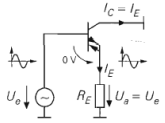
\includegraphics[width=4.00cm]{img_64.png}
\end{figure}
\begin{figure}[H]
\centering
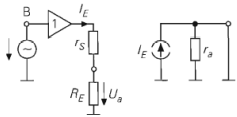
\includegraphics[width=5.00cm]{img_65.png}
\end{figure}
\subsubsection{Collecteur et émetteur connectés}
Comme le transistor diamant est alimenté de manière externe, on peut le faire fonctionner de la manière suivante (avec le courant qui sort "de nulle part")
\begin{figure}[H]
\centering
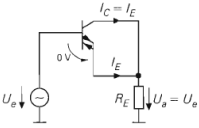
\includegraphics[width=4.00cm]{img_66.png}
\end{figure}
\begin{figure}[H]
\centering
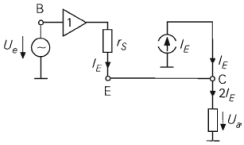
\includegraphics[width=5.00cm]{img_67.png}
\end{figure}
\subsubsection{Couplage sur la base}
\begin{figure}[H]
\centering
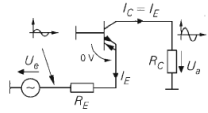
\includegraphics[width=5.00cm]{img_68.png}
\end{figure}
\begin{figure}[H]
\centering
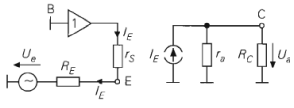
\includegraphics[width=5.00cm]{img_69.png}
\end{figure}
\paragraph{Circuit d'addition}
\begin{figure}[H]
\centering
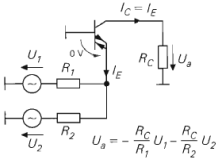
\includegraphics[width=5.00cm]{img_70.png}
\end{figure}
\paragraph{Circuit de soustraction}
\begin{figure}[H]
\centering
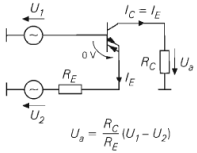
\includegraphics[width=5.00cm]{img_71.png}
\end{figure}
\subsubsection{Amplificateur différentiel}
\begin{figure}[H]
\centering
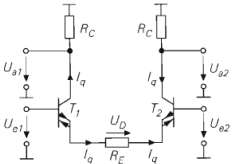
\includegraphics[width=5.00cm]{img_72.png}
\end{figure}
\begin{figure}[H]
\centering
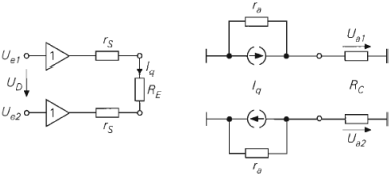
\includegraphics[width=6.00cm]{img_73.png}
\end{figure}
\subsubsection{Gyrateur}
Équivalent d'un transformateur mais qui fonctionne en DC
$$I_1=\frac{1}{R_G}U_2$$
$$I_2=\frac{1}{R_G}U_1$$
\begin{figure}[H]
\centering
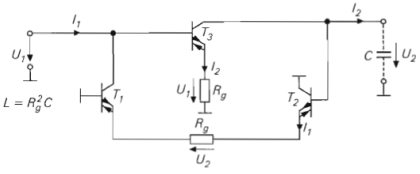
\includegraphics[width=6.00cm]{img_74.png}
\end{figure}
\subsubsection{Intégrateur}
\begin{figure}[H]
\centering
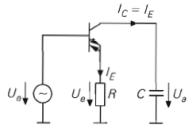
\includegraphics[width=5.00cm]{img_75.png}
\end{figure}
\begin{figure}[H]
\centering
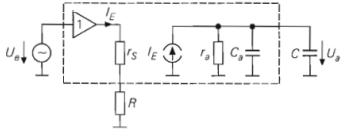
\includegraphics[width=6.00cm]{img_76.png}
\end{figure}
$r_a(C_a+C)$ représente la limite de fréquence basse de l'intégrateur. Il n'y a quasiment pas de limite haute ($f_T$)
\subsection{Terminaisons de lignes de transmissions}
\begin{figure}[H]
\centering
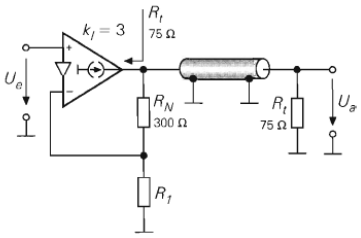
\includegraphics[width=6.00cm]{img_77.png}
\end{figure}
\subsection{Driver de ligne coax}
\begin{figure}[H]
\centering
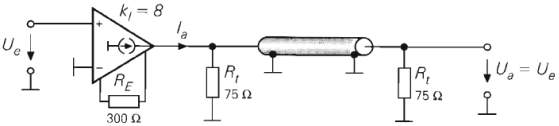
\includegraphics[width=\columnwidth]{img_55.png}
\end{figure}
$$U_a=\frac{1}{2}I_aR_w=\frac{k_1R_w}{2R_E}U_e$$
$$R_e\approx\frac{k_1}{2}R_2$$
\end{multicols}
\end{document}